%%=============================================================================
%% Methodologie
%%=============================================================================

\chapter{\IfLanguageName{dutch}{Methodologie}{Methodology}}
\label{ch:methodologie}

%% TODO: Hoe ben je te werk gegaan? Verdeel je onderzoek in grote fasen, en
%% licht in elke fase toe welke stappen je gevolgd hebt. Verantwoord waarom je
%% op deze manier te werk gegaan bent. Je moet kunnen aantonen dat je de best
%% mogelijke manier toegepast hebt om een antwoord te vinden op de
%% onderzoeksvraag.

\section{Datasets}
\label{sec:datasets}

De keuze van de dataset is belangrijk. Dit onderzoek wil de capaciteiten van AutoML systemen testen op realistische situaties. De traditionele datasets (CIFAR, MNIST ...) waarmee deze algoritmen getraind zijn vallen onmiddellijk uit de selectie zoals uitgelegd in sectie \ref{subsec:autokeras}.

\subsection{Cats vs dogs}
\label{subsec:catsvsdogs}

\begin{figure}
    \begin{subfigure}{.5\textwidth}
        \centering
        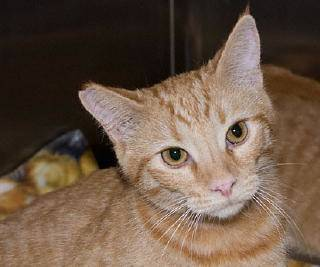
\includegraphics[width=.8\linewidth]{img/good_cat.jpg}
        \label{fig:cat-goog}
    \end{subfigure}%
    \begin{subfigure}{.5\textwidth}
        \centering
        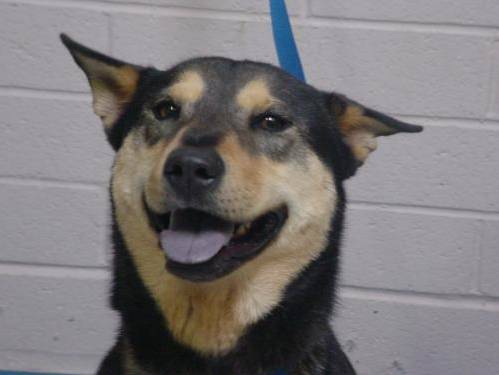
\includegraphics[width=.8\linewidth]{img/good_dog.jpg}
        \label{fig:dog-good}
    \end{subfigure}
    \caption{Kat en hond zijn de focus van de afbeelding.}
    \label{fig:catdog-good}
\end{figure}

\begin{figure}
    \begin{subfigure}{.5\textwidth}
        \centering
        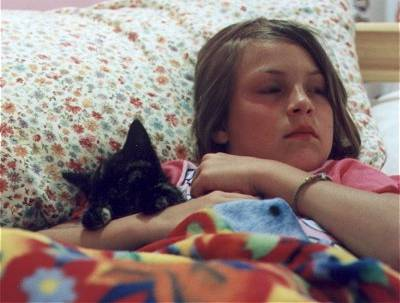
\includegraphics[width=.8\linewidth]{img/bad_cat.jpg}
        \label{fig:cat-bad}
    \end{subfigure}%
    \begin{subfigure}{.5\textwidth}
        \centering
        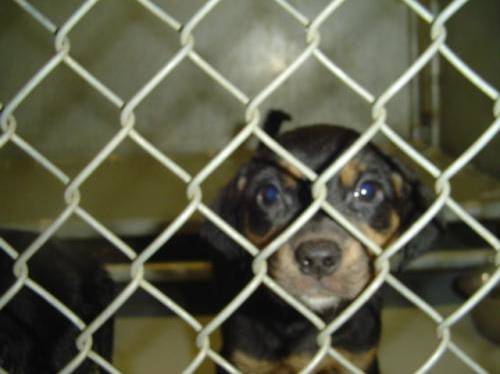
\includegraphics[width=.8\linewidth]{img/bad_dog.jpg}
        \label{fig:dog-bad}
    \end{subfigure}
    \caption{Kat en hond zijn niet de focus van de afbeelding.}
    \label{fig:catdog-bad}
\end{figure}

Een eerste testronde wordt uitgevoerd met een online\footnote{\url{https://www.kaggle.com/c/dogs-vs-cats/data}} dataset over katten en honden. Ooit was de dataset het onderwerp van een \textit{data science} wedstrijd en mogen vrij gebruikt worden. Ze bestaat uit 250000 foto's die gelijkaardig zijn aan de afbeeldingen in figuur \ref{fig:catdog-good}. Er is niks van \textit{preprocessing} toegepast, de foto's kunnen dus evengoed op uw smartphone staan. Door realistische foto's te gebruiken introduceren we een nieuwe moeilijkheid voor de optimalisatiealgoritmen, zo moet het ook rekening houden met volgende zaken: 

\begin{itemize}
    \item Foto's kunnen zeer verschillende resoluties hebben.
    \item De kleuren zijn in 3 dimensies (rood, groen, blauw).
    \item Door het originele formaat te behouden en de afbeelding niet te knippen naar het dier zelf, kan het zijn dat de focus van de afbeelding niet op het dier ligt (zie afbeeldingen in figuur \ref{fig:catdog-bad}).
\end{itemize}

Onduidelijke foto's zijn in de minderheid maar handig om te ontdekken waaraan het model gevoelig is.

Omdat de \textit{dataset} gebruikt is in een wedstrijd zijn er honderden inzendingen beschikbaar van mensen die een poging gedaan hebben om het probleem op te lossen. Een vergelijking van performantie met onze geautomatiseerde modellen tegenover modellen die door een persoon zijn samengesteld is op zijn plaats.

\subsection{FFMPEG}
\label{subsec:ffmpeg}
